\documentclass[10pt, landscape]{article}
\usepackage[scaled=0.92]{helvet}
\usepackage{calc}
\usepackage{graphicx}
\usepackage{multicol}
\usepackage{ifthen}
\usepackage[a4paper,margin=3mm,landscape]{geometry}
\usepackage{amsmath,amsthm,amsfonts,amssymb}
\usepackage{color,graphicx,overpic}
\usepackage{hyperref}
\usepackage{newtxtext} 
\usepackage{enumitem}
\usepackage{graphicx}
\usepackage[table]{xcolor}
\usepackage{mathtools}
\usepackage[document]{ragged2e}
\usepackage{listings}
\setlist{nosep}
\usepackage{subfig}


% for including images
\graphicspath{ {./images/} }


\pdfinfo{
  /Title (CS3223.pdf)
  /Creator (TeX)
  /Producer (pdfTeX 1.40.0)
  /Author (Pei Cheng Yi)
  /Subject (CS3223)
  /Keywords (CS3223, nus,cheatsheet,pdf)}

% Turn off header and footer
\pagestyle{empty}

\newenvironment{tightcenter}{%
  \setlength\topsep{0pt}
  \setlength\parskip{0pt}
  \begin{center}
}{%
  \end{center}
}

% redefine section commands to use less space
\makeatletter
\renewcommand{\section}{\@startsection{section}{1}{0mm}%
                                {-1ex plus -.5ex minus -.2ex}%
                                {0.5ex plus .2ex}%x
                                {\normalfont\large\bfseries}}
\renewcommand{\subsection}{\@startsection{subsection}{2}{0mm}%
                                {-1explus -.5ex minus -.2ex}%
                                {0.5ex plus .2ex}%
                                {\normalfont\normalsize\bfseries}}
\renewcommand{\subsubsection}{\@startsection{subsubsection}{3}{0mm}%
                                {-1ex plus -.5ex minus -.2ex}%
                                {1ex plus .2ex}%
                                {\normalfont\small\bfseries}}%
\renewcommand{\familydefault}{\sfdefault}
\renewcommand\rmdefault{\sfdefault}
%  makes nested numbering (e.g. 1.1.1, 1.1.2, etc)
\renewcommand{\labelenumii}{\theenumii}
\renewcommand{\theenumii}{\theenumi.\arabic{enumii}.}
\renewcommand\labelitemii{•}
\renewcommand\labelitemiii{•}
%  convenient absolute value symbol
\newcommand{\abs}[1]{\vert #1 \vert}
%  convenient floor and ceiling
\newcommand{\floor}[1]{\lfloor #1 \rfloor}
\newcommand{\ceil}[1]{\lceil #1 \rceil}
%  convenient modulo
\newcommand{\Mod}[1]{\ \mathrm{mod}\ #1}
%  for logical not operator, iff symbol, convenient "if/then"
\renewcommand{\lnot}{\mathord{\sim}}
\let\then\Rightarrow
\let\Then\Rightarrow
%  vectors
\newcommand{\vv}[1]{\boldsymbol{#1}}
\newcommand{\VV}[1]{\overrightarrow{#1}}
%  column vector
\newcommand{\cvv}[1]{\left(\begin{smallmatrix}#1\end{smallmatrix}\right)}
\newcommand{\code}[1]{\textcolor{myblue}{\texttt{#1}}}
\newcommand\bggreen{\cellcolor{green!10}}

\makeatother
\definecolor{myblue}{cmyk}{1,.72,0,.38}
\everymath\expandafter{\the\everymath \color{myblue}}
% Define BibTeX command
\def\BibTeX{{\rm B\kern-.05em{\sc i\kern-.025em b}\kern-.08em
    T\kern-.1667em\lower.7ex\hbox{E}\kern-.125emX}}

% Don't print section numbers
\setcounter{secnumdepth}{0}

\setlength{\parindent}{0pt}
\setlength{\parskip}{0pt plus 0.5ex}
%% this changes all items (enumerate and itemize)
\setlength{\leftmargini}{0.5cm}
\setlength{\leftmarginii}{0.4cm}
\setlength{\leftmarginiii}{0.5cm}
\setlist[enumerate,1]{leftmargin=2mm,labelindent=1mm,labelsep=1mm}
\setlist[itemize,1]{leftmargin=2mm,labelindent=1mm,labelsep=1mm}
\setlist[itemize,2]{leftmargin=3mm,labelindent=1mm,labelsep=1mm}
\setlist[itemize,3]{leftmargin=3mm,labelindent=1mm,labelsep=1mm}

%My Environments
\newtheorem{example}[section]{Example}
% -----------------------------------------------------------------------

\begin{document}
\raggedright
\footnotesize
\begin{multicols}{4}


% multicol parameters
% These lengths are set only within the two main columns
\setlength{\columnseprule}{0.25pt}
\setlength{\premulticols}{1pt}
\setlength{\postmulticols}{1pt}
\setlength{\multicolsep}{1pt}
\setlength{\columnsep}{2pt}

\begin{center}
    \fbox{%
        \parbox{0.8\linewidth}{\centering \textcolor{black}{
            {\Large\textbf{CS3223}}
            \\ \normalsize{AY22/23 Sem 2}}
            \\ {\footnotesize \textcolor{myblue}{github.com/SeekSaveServe}}
        }%
    }
\end{center}

% COMMENTED OUT FOR FINALS
% \subsection{L1 - Data Storage}
% \textbf{Magnetic Disks} \newline

% 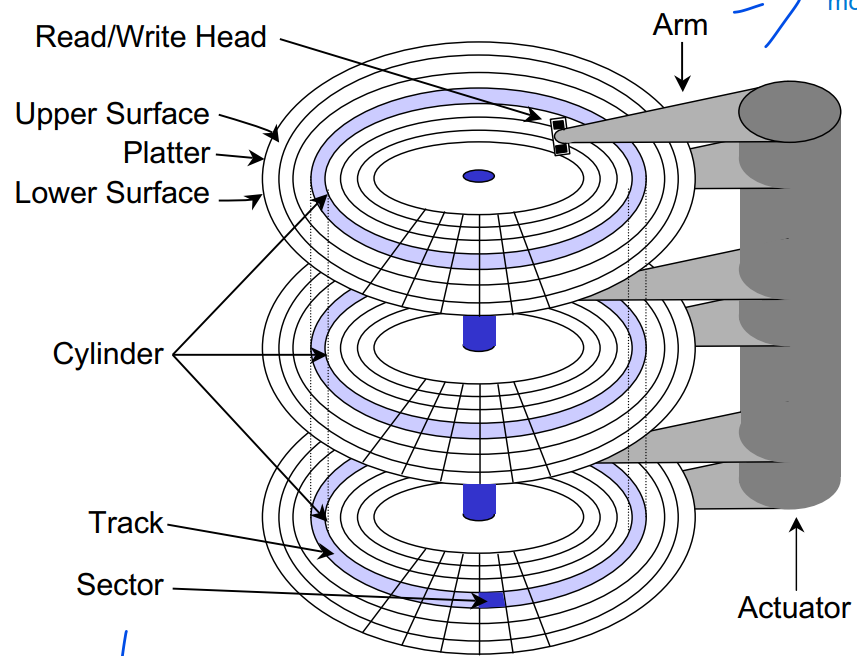
\includegraphics[width=3.5cm, height =2cm]{magnetic_disk.png}

% \begin{itemize}
%     \item \textbf{Disk Access Time} Seek time + Rotational Latency + Transfer time
%     \item \textbf{Response time} Queueing delay + Disk access time
%     \item \textbf{Rotational Delay} $\frac{1}{2} \frac{60s}{RPM}$ 
%     \item \textbf{Transfer Time} sectors on the same track * $\tfrac{Time Per Revolution}{Sectors Per Track}$
% \end{itemize}

% \textbf{Buffer Manager}
% \begin{itemize}
%   \item \textbf{Buffer pool} Main memory allocated for DBMS
%   \item \textbf{pin count} is incremented upon pinning
%   \item \textbf{dirty bit} is updated when the page is unpinned (if modified)
%   \item \textbf Replacement is only possbile if pin count == 0 
% \end{itemize}

% 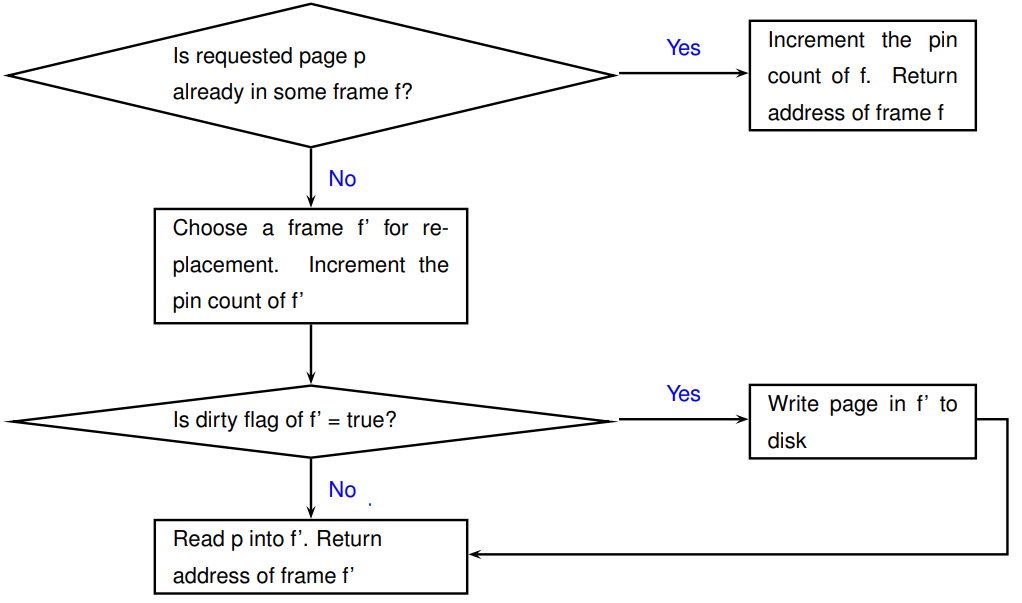
\includegraphics[width=5cm, height =3cm]{buff_manager_handle_request.png}

% \textbf{Replacement Policies}
% \textbf{LRU Policy}
% \begin{itemize}
%   \item Maintains a queue of pointers to frames with pin count = 0
% \end{itemize}


% \textbf{Clock Replacement Policy}
% \includegraphics*[width=5cm, height=3cm]{clock.png}
% \begin{itemize}
%   \item Simplifies LRU with a second chance round robin system
%   \item Each frame has a \textcolor{red}{reference bit} that is turned on when pin count reaches 0
%   \item Repalces a page when referenced bit if off and pin count is 0
% \end{itemize}

% \textbf{File Organisation}
% \includegraphics*[width=7cm, height=3cm]{heap_file.png}

% \textbf{Page Formats: Fixed Length Records}
% \begin{itemize}
%   \item \textbf{Packed Organisation} Store records in contiguous slots
%   \item \textbf{Unpacked Organisation} Uses a bit array to maintain free slots
% \end{itemize}

% \includegraphics*[width=5cm, height=2.5cm]{page_org.png}


% \textbf{Page Formats: Slotted Page (variable length record)}
% \begin{itemize}
%   \item Store records in slots of \textsl{(record offset, record length)}
%   \item Record Offset: Offset of the record from the start of the page
% \end{itemize}

% \begin{multicols}{2}
%   \begin{itemize}
%     \item 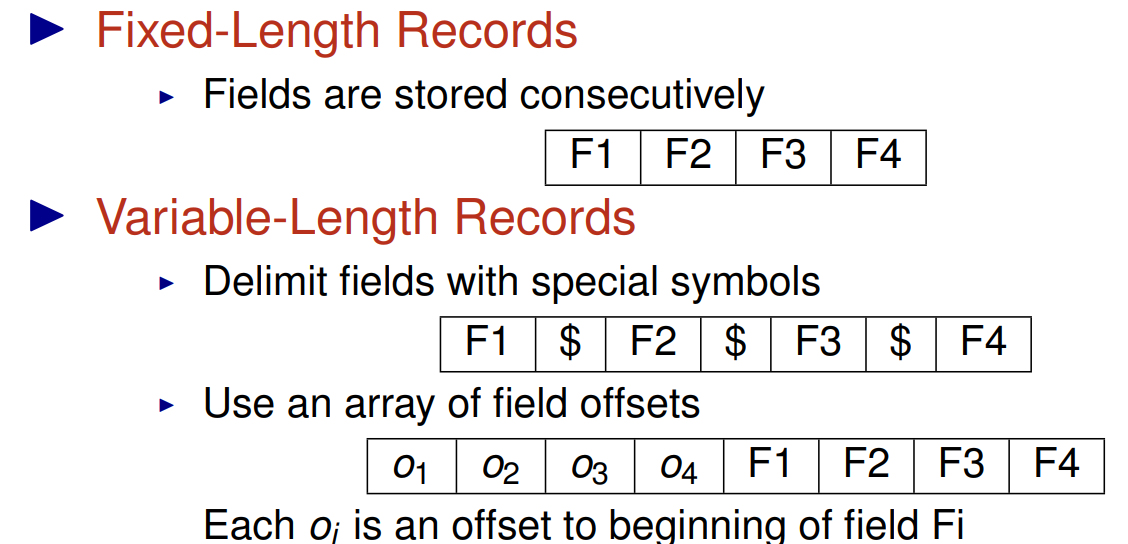
\includegraphics[width=3.5cm, height=2cm]{var_record.png}
%   \end{itemize}  
%   \begin{itemize}
%     \item \includegraphics*[width=4cm, height=3cm]{slot_page.png}
%   \end{itemize}
% \end{multicols}


% \subsection{L2 And L3 - Indexing}
% \begin{itemize}
%   \item A search key is a sequence of k attributes. If k > 1, composite key
%   \item A search key is an unique index if it is a candidate key
%   \item An index is stored as a file
% \end{itemize}

% \textbf{Format of data entries}
% \begin{itemize}
%   \item Format 1: k* is an actual data record with search value k
%   \item Format 2: k* is the form (k, rid)
%   \item Format 3: k* is the form (k, rid-list*)
%   \item Note: Different formats affects the number of data entries stored in a page
% \end{itemize}

% \textbf{Clustered Vs Unclustered}
% \begin{itemize}
%   \item \textcolor{red}{Clustered}: Order of data entries is the same as the oreder of data records. Can only be built on ordered field (e.g. primary key)
%   \item \textcolor{green}{Unclustered}: Order of data entries does not correspond to the order of data records
%   \item The implication is that we can read an entire clustered page with 1 I/O
%   \item  B+ Tree: Format 1 is clustered, Format 2 and 3 can be clustered if data records are sorted on the search key
%   \item Hash: Only format 1 is clustered since hashing do not store data entries in search key order
% \end{itemize}

% \textbf{Tree Based Index - B+ Tree}
% \begin{itemize}
%   \item Leaf nodes are doubly linked and store Data Entries
%   \item Internal nodes sotre index entries (p0, k, p1 ... pk, k, pk+1)
%   \item Internal nodes contains m entries,  m $\in$ [d, 2d] $\rightarrow$ space utilisation $\geq$ 50\%
%   \item Root contains m entries, m $\in$ [1, 2d]
% \end{itemize}

% \textbf{B+ Tree - Split Overflow Nodes}
% \begin{itemize}
%   \item Distribute d+1 entries to the new leaf node
%   \item Create new entry index using smallest key in the new node (middle key)
%   \item Insert new entry into parent node of overflowed node
% \end{itemize}
% 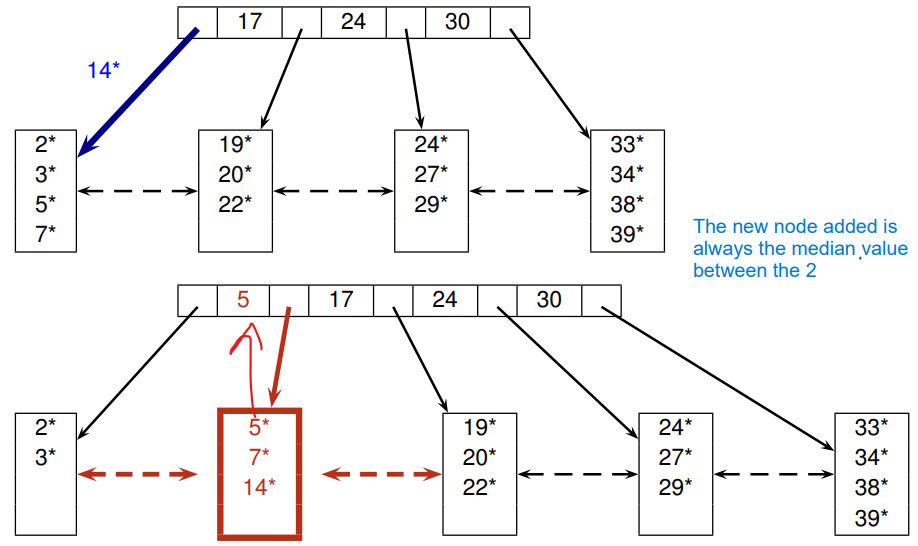
\includegraphics[width=7cm, height=4cm]{split_overflow_node.png}

% \textbf{B+ Tree - Overflow Propagation}
% \newline
% 5 is pushed up
% 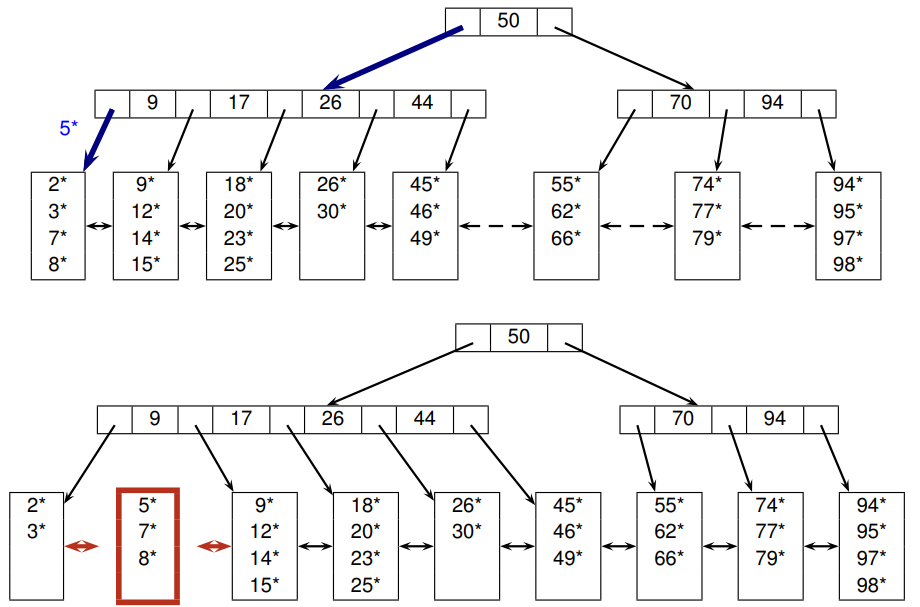
\includegraphics[width=7cm, height=4cm]{overflow_progpagation1.png}
% 17 is pushed up
% 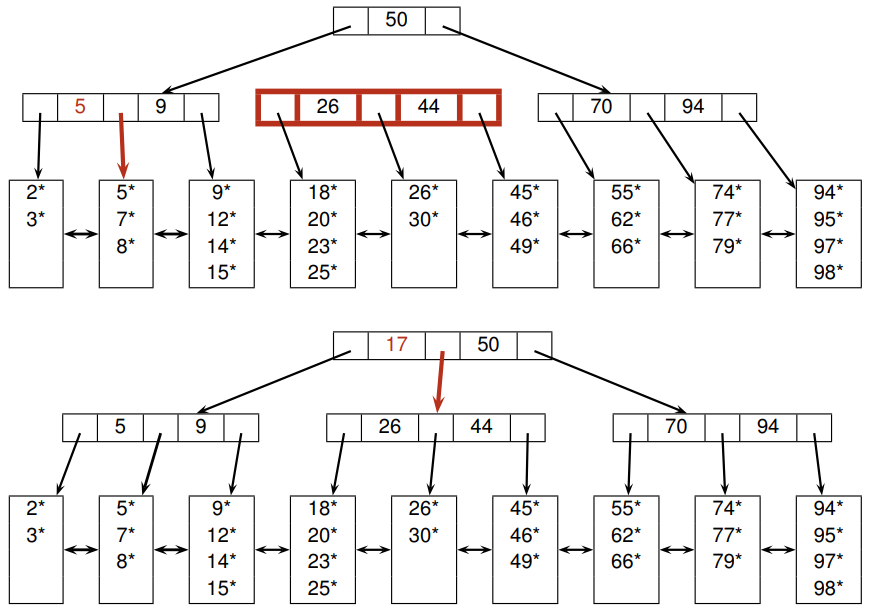
\includegraphics[width=7cm, height=4cm]{overflow_progpagation2.png}
% Excess middle node is pushed updated to parent node \newline


% \textbf{B+ Tree - Redistribution of data entries} \newline
% Two nodes are siblings if they have the same parent node \newline

% 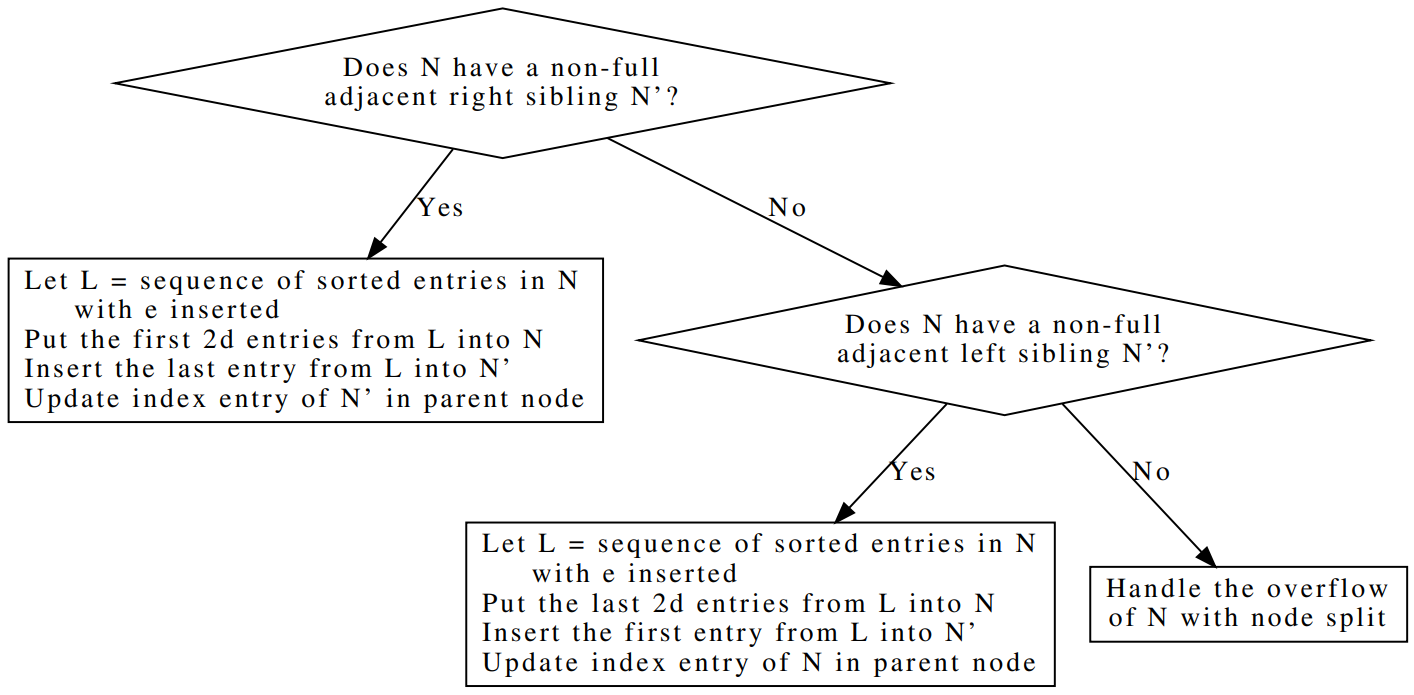
\includegraphics[width=7cm, height=3cm]{overflow_redistribution.png}

% \textbf{B+ Tree - Underflow}
% \begin{itemize}
%   \item Underflow occurs when a node has less than d entries
%   \item Underflow is resolved by redistributing entries between siblings
%   \item An underflow node is merged if each of its adjacent siblings have exactly d entries
% \end{itemize}

% 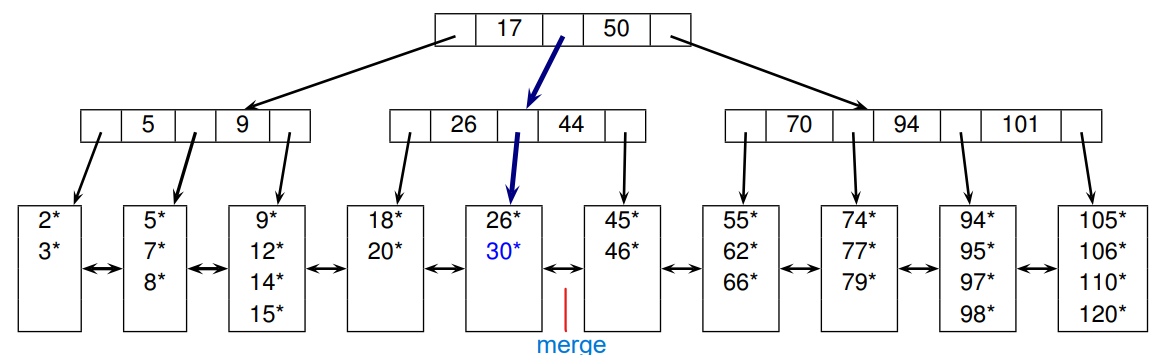
\includegraphics[width=7cm, height=2cm]{merge_nodes.png}
% 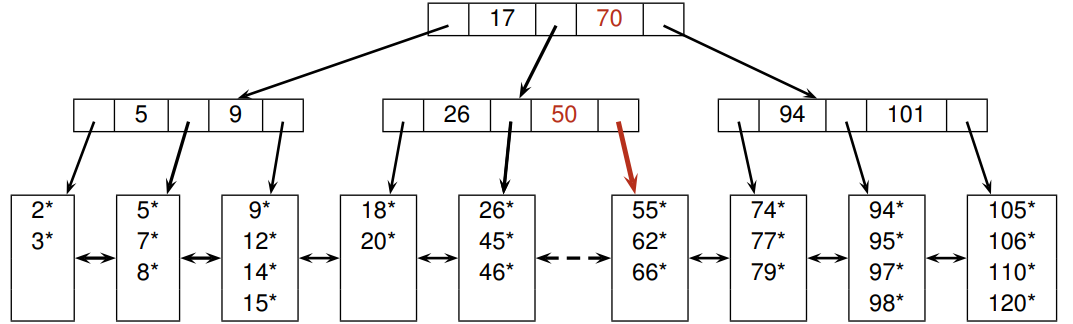
\includegraphics[width=7cm, height=2cm]{merge_parent.png}

% \textbf{B+ Tree - Bulk Loading}
% \begin{itemize}
%   \item Initiazing a B+ tree by insertion is expensive (need to traverse tree n times)
%   \item 1. Sort all data entries by search key
%   \item 2. Initialise B+ tree with an empty root page
%   \item 3. Load data entries into leaf pages 
%   \item 4. In asc order, insert the index entry of each leaf page into the rightmost parent node
% \end{itemize}


% \textbf{Hash Based Index}
% \begin{itemize}
%   \item Does not support range search, only equality queries
% \end{itemize}

% \textbf{Static Hashing}
% \begin{itemize}
%   \item N buckets, each bucket has 1 primary page and $\geq$ 0 overflow pages
%   \item To maintain performance, we need to routinely construct bigger hash tables and redistribute data entries
% \end{itemize}

% \textbf{Dynamic Hashing - Extendible Hashing}
% \begin{itemize}
%   \item No overflow pages! A bucket can be thought of as a page
%   \item At most 2 Disk I/Os for equality search (at most 1 if directory and bucket fits in memory)
%   \item Instead of maintaining data entries, we maintain pointers to data entries in buckets
%   \item Instead of maintaining buckets, maintain a directory of pointers to buckets
%   \item The directory has $2^d$ buckets, where d is the global depth --> large overhead if hashing is uniform
%   \item Each director entry diffets by a unique d-bit adddress
%   \item Two directories are corresponding iff their addresses differ only in the dth bit
%   \item All entries with the same local depth (l) have the same last l bits in h(k)
% \end{itemize}

% 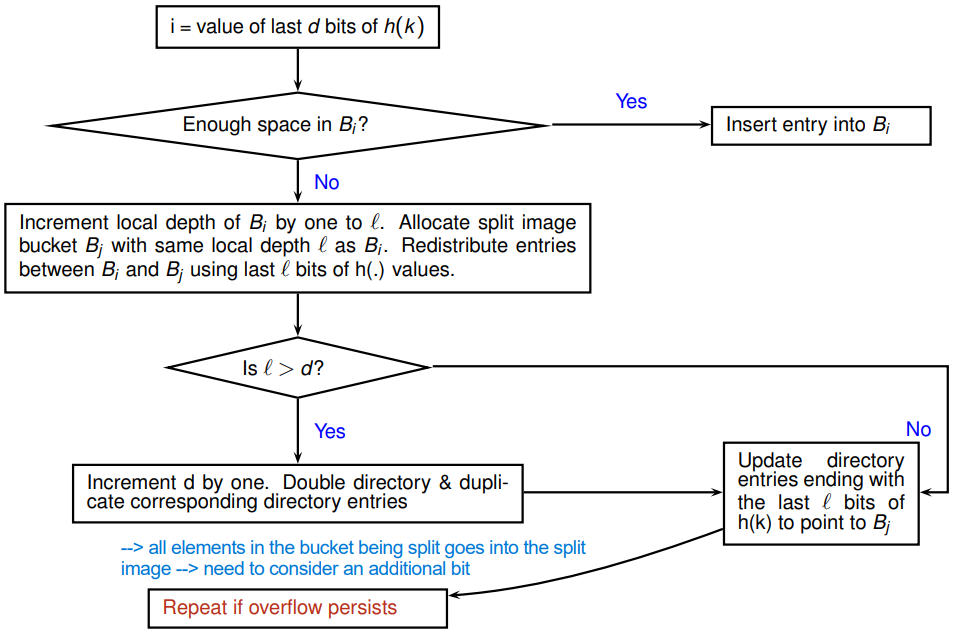
\includegraphics[width=7cm, height=4cm]{extendible_hash.png}
% \textbf{Extendible Hashing - Split, Double}
% \begin{itemize}
%   \item Split and doubling is checked every time a bucket is full 
%   \item Doubling only happens if local depth = global depth
%   \item The split image has the same depth as the split bucket
%   \item Other than the split image of the split bucket, split image of other buckets points to the same corresponding bucket
%   \item Each bucket is pointed by $2^(d-l)$ directories
% \end{itemize}

% \textbf{Extendible Hashing - Deletion}
% \begin{itemize}
%   \item $B_i$ is deallocated
%   \item l decrement by 1
%   \item Directory Entries that point to $B_i$ points to its corresponding bucket
% \end{itemize}

% \textbf{Dynamic Hashing - Linear Hashing}
% 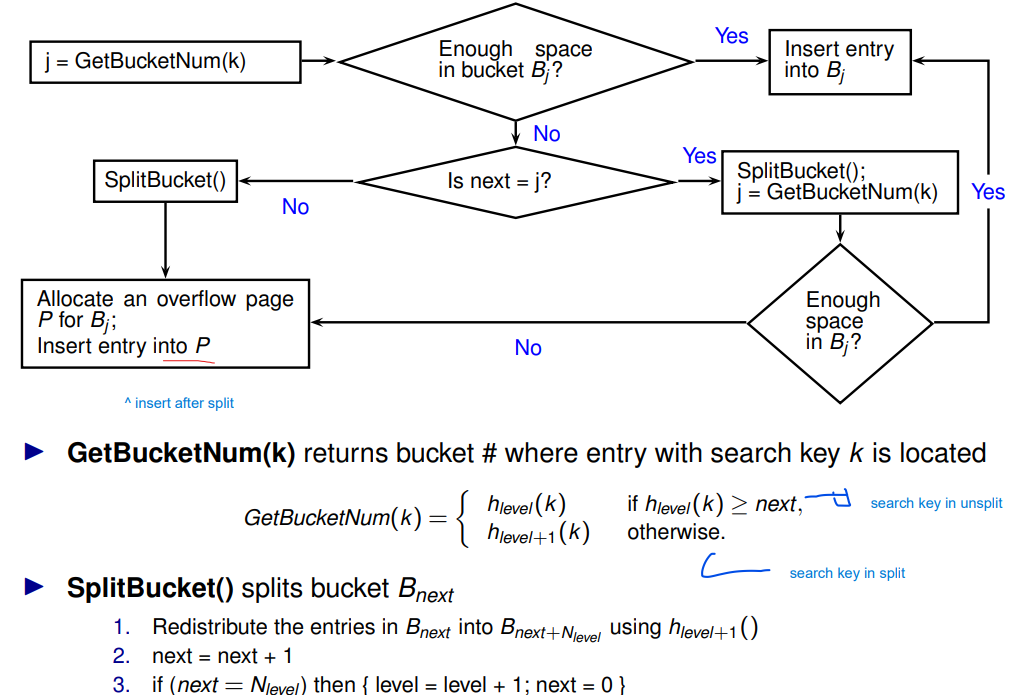
\includegraphics[width=7cm, height=4cm]{linear_hash.png}  
% \begin{itemize}
%   \item One I/O for equality search (more per number of overflow pages in bucket)
%   \item Performs worse than extendible hashing if distribution is skewed
%   \item Does not require a directory
%   \item Higher average space utilisation, but longer overflow chains
%   \item Has a family of hash functions, with each having a range twice of its predecessor
%   \item $N_0$: initial number of buckets
%   \item $N_i = 2^i N_0$: number of buckets at start of round i
%   \item $next$: the next bucket to be split, this is incremented every time split happnes
%   \item $h_{i+1}=h(k) mod N_{i+1}$: hash function for round i, if the bucket $>$ next (already split)
%   \item $h_{i}=h(k) mod N_{i}$: hash function for round i+1, if the bucket $>$ next
%   \item Split Citeria: By default, split when a bucket overflows
% \end{itemize}

% \textbf{Linear Hashing - Deletion}
% \begin{itemize}
%   \item Essentially the inverse of insertion
%   \item If the last bucket is empty $\rightarrow$ delete it,  $next$--
%   \item If $next$ is 0, set it to $M/2 - 1$, and we can decrement level by 1 (half of buckets have been deleted if $next$ is 0)
%   \item Merging with corresponding bucket is optional
% \end{itemize}

\subsection{L4: Query Evaluation - Sort, Select}
% \textbf{Sorting - External Merge Sort}
% \newline
% Projection, join, bulk loading etc all require sorting

% 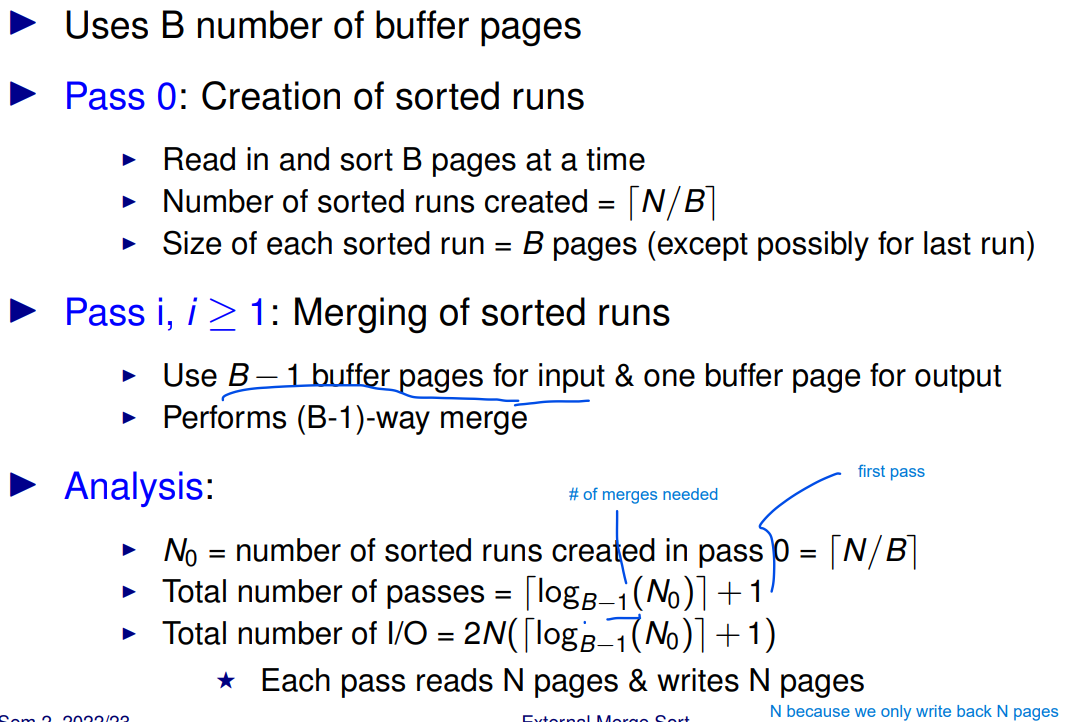
\includegraphics[width=7cm, height=4cm]{ext_sort.png}

\textbf{External Merge Sort - Bocked I/O}
\begin{itemize}
  \item Read and write in blocks of \textbf{b} buffer pages (replace b with 1 for unoptimised)
  \item $\floor{\frac{B-b}{b}}$ blocks for input, 1 block for output
  \item Can merge at most $\floor{\frac{B-b}{b}}$ sorted runs in each merge pass
  \item $F=\floor{\frac{B}{b}} - 1$ runs can be merged at each pass
  \item Num passes = $\log_{F} N_0$
  \item New cost: $2N(\ceil{\log_{F} N_0} + 1)$
\end{itemize}

\textbf{B+ tree sort}
\begin{itemize}
  \item B+ Tree is sorted by key
  \item Format 1 (clustered): Sequential Scan 
  \item Format 2/3:Retrieve data using RID for each data entry 
  \item Unclustered implies more I/Os
\end{itemize}

\textbf{Access Path} refers to the different ways to retrieve tuples from a relation. It is either a \textbf{\textcolor{red}{file scan}} or a \textbf{\textcolor{green}{index plus matching selection condition}}. The more \textbf{selective} the access paths, the fewer pages are read from the disk.
\begin{itemize}
  \item Table scan: scan all data pages 
  \item Index scan: scan all index pages 
  \item Table intersection: combine results from multiple index scans (union, intersec). Find RIDs of each predicate and get the intersection
\end{itemize}

\textbf{Query: Selection}
\textbf{Covering Index}
\begin{itemize}
  \item I is a covering index of $query_Q$ if I contains all attributes of Q
  \item No RID lookup is needed, Index-only plan
  \item If data is unclustered, unsorted, no index $\rightarrow$ best way is to collect all entries and sort by RID before doing I/O 
\end{itemize}

\textbf{CNF Predicate}
\begin{itemize}
  \item Find RIDs of each predicate and get the intersection
  \item Conjuncts are in the form (R.A op c V R.a op R.b) 
  \item CNF are conjuncts (or terms) connected by $\land$ 
\end{itemize}

\textbf{Matching Predicates - B+ Tree}
\begin{itemize}
  \item Non-disjunctive CNF (no $\lor$)
  \item At most one non-equality comparison operator which must be on the \textbf{last attribute in the CNF}
  \item $(k_1=c_1) \land (k_2=c_2) \land ...k_i op c_i | I=(k_1, k_2...k_n)$ 
  \item The order of k matters, and there cannot be missing $K_i$ in the middle of the CNF
  \item Having inequality operator before equality operator makes the query to be less selective 
\end{itemize}

\textbf{Matching Predicates - Hasing}
\begin{itemize}
  \item No inequality operators $(k_1=c_1) \land ... k_i =c_n | I=(k_1, k_2...k_n)$
  \item Unlike B+ tree, \textbf{all predicates must match}
\end{itemize}

I=(age, weight, height), p=($age \geq 20 \land age \geq 18 weight=50 \land height=150 \land level=3$) \newline
\textbf{Primary Conjuncts} : The subset of conjuncts in p that I matches \newline
Primary Conjuncts: $age \geq 20 \land age \geq 18$ \newline
\textbf{Covered Conjuncts} : The subset of conjuncts in p that I covers (conjuncts that appear in I). Primary conjunct $\subseteq$ covered conjunct \newline
Covered Conjuncts: $age \geq 20 \land age \geq 18 \land height=150$ \newline

\textbf{Cost Notation}  \newline
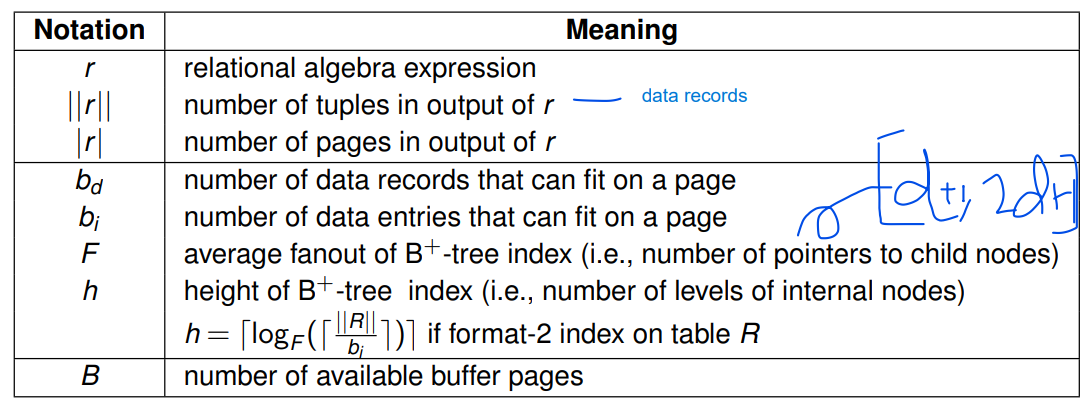
\includegraphics[width=4cm, height=2cm]{notation.png}

\textbf{Cost of B+-tree index evaluation of p} \newline
Let p'=primary conjuncts of p (\textbf{matching}) | $p_c$=covered conjuncts of p \newline
\begin{itemize}
  \item[1.] Navigate internal nodes to locate the first leaf page
  $$
  Cost_{internal} = \left\{
    \begin{array}{ll}
        \ceil{log_F(\ceil{\frac{||R||}{b_d}})} | Format 1 \\
        \ceil{log_F(\ceil{\frac{||R||}{b_i}})} | Otherwise
    \end{array}
\right.
  $$ \newline
  \item[1.1] This is traversing the height of B+ tree
  \item[2.] Scan leaf pages to access all qualifying data entries
  $$
  Cost_{leaf} = \left\{
    \begin{array}{ll}
        {\ceil{\frac{||\sigma_{p'}(R)||}{b_d}}} | Format 1 \\
        {\ceil{\frac{||\sigma_{p'}(R)||}{b_i}}} | Otherwise
    \end{array}
\right.
  $$ \newline
  \item This is the cost of reading qualifying conjuncts
  \item Using $p_c$ would be wrong since covering conjuncts may be non-matching which results in more reads from the leaves. 
  \item Conversely, non-matching (but covered) conjuncts cannot be derived from the B+ tree and needs to be read from disk
  \item Retrieve qualified data records using RID lookups. 0 if I is covering OR format 1 index. $||\sigma_{p_c}(R)||$ otherwise
  \item includegraphics[width=5cm, height=1.3cm]{optimisation.png}
\end{itemize}

\textbf{Cost of Hash index evaluation of p (all covered index are matched)} \\
\begin{itemize}
  \item Format 1: cost to retrieve \textbf{data entries} is at least$\ceil{\frac{||\sigma_{p'}(R)||}{b_d}}$
  \item Format 2: cost to retrieve \textbf{data entries} is at least $\ceil{\frac{||\sigma_{p'}(R)||}{b_i}}$
  \item Format 2: Cost to retrieve \textbf{data records} is 0 if it is a covering index (all information in data entry) OR $||\sigma_{p'}(R)||$ otherwise
\end{itemize}

\subsection{L5:Query Evaluation - Projection and Join}
\begin{itemize}
  \item $\pi^*(R)$ refers to projection without removing duplicates
  \item $\pi(R)$ involves 1.Removing unwanted attributes 2. Removing duplicates
  \item Sorting is better if we have many duplicates or if hte distribution is nonuniform(overflow more likely for hashing paritions)
  \item Sorting allows results to be sorted
  \item If $B > \sqrt{|\pi^*_L(R)|}$, then both sorting and hashing has similar I/O costs ($\ceil{\frac{\ceil{R}}{B}} \rightarrow |R| + 2*|\pi^*_L(R)|$)
\end{itemize} 

\textbf{Approach 1: project based on sorting}\\
\begin{itemize}
  \item \textbf{\color{red}{Naive}}: Extract attributes L from records $\rightarrow\pi^*_L(R) \rightarrow$ Sort attributes $\rightarrow$ Remove duplicates
  \item Cost: Cost to scan records ($|R|$) + Cost to output to temporary result ($|\pi^*_L(R)|$) $\rightarrow$ cost to sort records ($2|\pi^*_L(R)|\log_m(N_0)+1$) $\rightarrow$ Cost to scan data records $|\pi^*_L(R)|$
  \item \textbf{\color{green}{Optimisation}}: Create Sorted runs with attributes L only (Pass 0) $\rightarrow$ Merge sorted runs and remove duplicates $\rightarrow$ $\pi_L(R)$ 
\end{itemize}

\textbf{Approach 2: project based on hashing}\\
\begin{itemize}
  \item Build a main-memory hash table to detect and remove duplicates. Insert to the hashtable if then entry is not already in it.
  \item 1. Partition R into $R_1, R_2...R_{B-1}$, hash on $\pi_L(t)$ for $t \in R$ $\leftarrow$ ($\pi^*_L(R_i)$ does not intersect $\pi^*_L(R_j), i!=j$)
  \item[1.1] Use 1 buffer for input and (B-1) for output
  \item[1.2] Read R 1 page at a time, and hash tuples into B-1 partitions
  \item[1.3] Flush output buffer to disk when full  
  \item 2. Eliminate duplicates in each partition $\pi^*_L(R_i)$
  \item $\pi_L(R)=\cup^{B-1}_i(\pi_L(R_i))$
  \item[2.1] For each partition, Initialise an in-memory hash table and insert each tuple into $B_j$ if $t \notin B_j$
\end{itemize}
\textbf{Parition overflow:} Hash table $\pi^*_L(R_i)$ is larger than available memory buffers. \newline
\textbf{Solution:} Recursively apply hash-based partitioning to overflowed partitions. \newline
\textbf{Analysis:} Effective (no overflow) when B $ > \frac{|\pi^*_L(R)|}{B-1} * f \approx \sqrt{f * \pi^*_L(R)|}$ \newline
If no partition overflow: (partition)$|R|+\pi^*_L(R)|$ + (duplicate elimination)$|\pi^*_L(R)|$ \newline


\textbf{Join} \\$R  \Join_\theta S$, where R is the outer relation and S is the inner relation

% \begin{multicols}{2}


    % \begin{itemize}

      % \item \textbf{Optimal join} \newline
      \textbf{Optimal join} \newline
      \begin{itemize}
        \item Cost: $|R| + |S|$
        \item load smaller relation into memory
        \item requires: $|S|+2$ buffers
      \end{itemize}

      % \item \textbf{Tuple-based} \newline
      \textbf{Tuple-based} \newline
      \begin{itemize}
        \item Cost: $|R| + ||R||*|S|$
        \item for each tuple r in R 
        \item for each tuple s in S 
        \item if (r matches s) then output $(r,s)$4 to result
      \end{itemize}

      % \item \textbf{Page-based} \newline
      \textbf{Page-based} \newline
      \begin{itemize}
        \item Load $P_R$ and $P_S$ to main memory
        \item Cost: $|R| + |R|*|S|$
        \item for each page $P_R$ in R 
        \item for each page $P_S$ in S
        \item for each tuple $r \in P_R$
        \item for each tuple $s \in P_S$ 
        \item if (r matches s) then output $(r,s)$4 to result
      \end{itemize}


      % \item \textbf{Block nested-loop} \newline
      \textbf{Block nested-loop} \newline
      \begin{itemize}
        \item Allocate 1 page for S, 1 for output, B-2 for R $|R| \le |S|$
        \item Cost:  $|R| + (\ceil{\frac{|R|}{B-2}} * |S|)$
        \item $|R|\le |S|$
        \item while Scanning R
        \item read next (B-2) pages of R to buffer
        \item for $P_S$ in S
        \item read $P_S$ into Buffer
        \item for $r \in buffer \land s \in P_S$
        \item if (r matches s) then output $(r,s)$4 to result
        \item Without materialisation: $\ceil{\frac{|R|}{B-2}}*|T|$
      \end{itemize}

      % \item \textbf{Index Nested Loop Join} \newline
      \textbf{Index Nested Loop Join} \newline
      \begin{itemize}
        \item There is an index on the join attributes of S
        \item Uniform distribution: r joins $\ceil{\frac{||S||}{||\pi_{B_j}(S)||}}$ tuples in S
        \item format 1 B+Tree:$|R| + ||R|| * J$
        \item Assuming unclustered:
        \item J = height of tree + reading leaf pages + RID Look up
        \item J = $\log_F(\ceil{\frac{||S||}{b_d}})$ (tree traversal)+$\ceil{\frac{||\pi_{p'}(S)||}{b_i}}$ (search leaf nodes) + RID lookup
        \item for $r \in R$ 
        \item use r to probe S's index to find matching tuples
      \end{itemize}

      % \item \textbf{Sort-Merge Join} \newline
      \textbf{Sort-Merge Join} \newline
      \begin{itemize}
        \item Sort R and S on join attributes and merge
        \item Cost: $2|\pi^*_L(R)|(\log_{B-1}(\frac{|R|}{B})+1)$ + $2|\pi^*_L(S)|(\log_{B-1}(\frac{|S|}{B})+1)$ + $|\pi^*_L(R)|+|\pi^*_L(S)|$
        \item merging cost is $|R|$ + $||R||*|S|$ if each tuple of R requires a full scan of S
        \item Optimisation: $B \ge N(R,i) + N(S,i) + 1 \ge \sqrt{|R|+|S|}$ 
        \item We can choose which relation to partition again if this is not met
        \item Cost: cost of getting R, S + k(write out ($|R|+|S|$)) + m(merge ($|R|+|S|$))
        \item If sorted on join column: $|R|+|S|$
      \end{itemize}

      % \item \textbf{Grace Hash Join} \newline
      \textbf{Grace Hash Join} \newline
      \begin{itemize}
        \item Partition into $B-1$ partitions
        \item If no partition overflow ($B > \sqrt{f*|S|}$):
        \item k(Cost to partition R, S) + Cost of probe phase
        \item Partition cost = cost of getting R + cost to write partitions($|R|$)
        \item Probe cost = $|R| + |S|$
      \end{itemize}

%     \end{itemize}
% \end{multicols}


% MID TERM CONTENT ENDS HERE
% \textbf{Sort-Merge Join: Optimised} \newline
% \begin{itemize}
%   \item Create sorted runs of R: Merge partially
%   \item Create sorted runs of S: Merge partially
%   \item Merge and join remaining sorted runs of R and S
% \end{itemize}
% Lecture 6
\subsection{L6: Query Optimisation}
\textbf{1. Search space: Queries considered} \\ 
\begin{itemize}
  \item \textbf{Search Place} Queries being considered
  \item \textbf{Linear} if at least one operand for each join is a base relation, bushy otherwise
  \item \textbf{Left-deep} if every right join operand is a base relation 
  \item \textbf{Right-deep} if every left join operand is a base relation
\end{itemize}

\textbf{2. Plan enumeration - for joins between 2 tables} \\
\begin{itemize}
  \item Basic DP is not always Optimal since it goes for lowest current cost and ignores the sorted property of outputs
  \item \textbf{Enhanced DP:} left-deep only, avoids cross products, considers early selection and projections, considers order of output
\end{itemize}
% 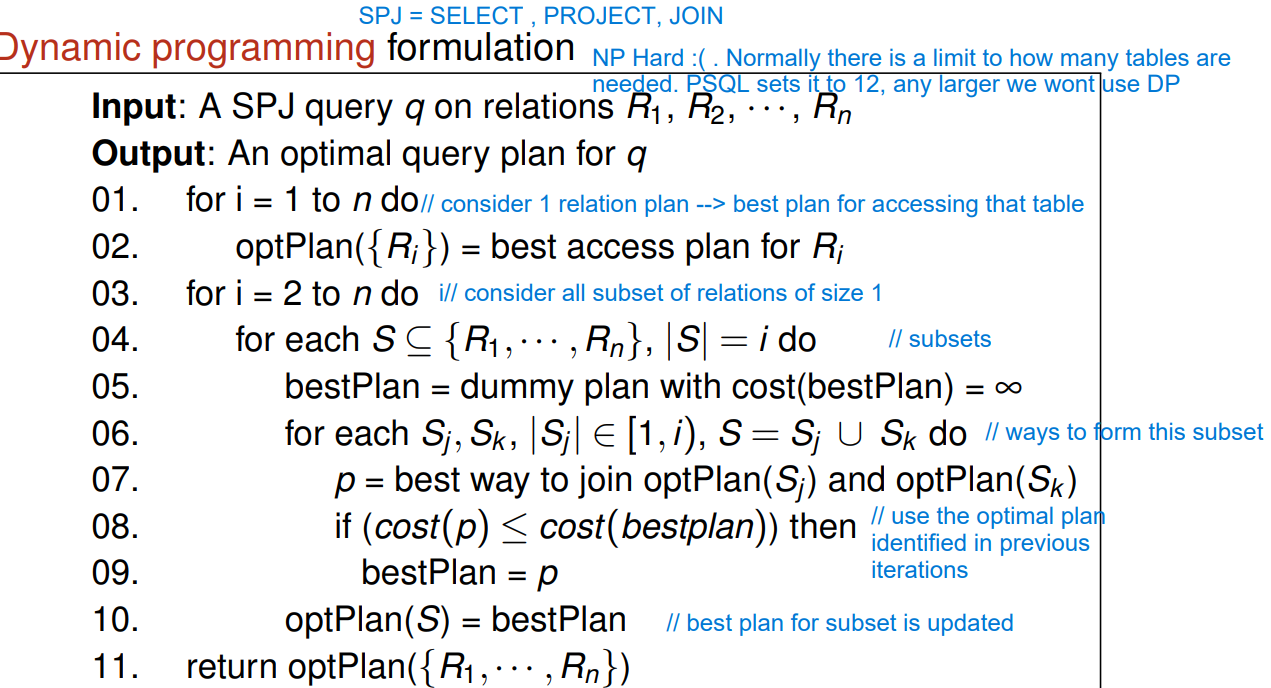
\includegraphics[width=7cm, height =3cm]{dp_2.png}

\textbf{3. Cost Model} \\
\begin{itemize}
  \item \textbf{Uniformity:} uniform distribution of all values
  \item \textbf{Independence:} Independent distribution of values in different attributes
  \item \textbf{Inclusion:} for $R\bowtie S, if ||\pi_A(R)|| \leq ||\pi_B(S)||$ then $\pi_A(R) \subseteq \pi_B(S)$
\end{itemize}

\textbf{Plans-no join, 1 table} \\
\begin{itemize}
  \item \textbf{Table scan} Scan the entire table. Cost: $|R|$
  \item \textbf{Index scan} Scan the index. Cost: 2 + $|$leaf pages satisfying the predicate$|$ + $||$entries satisfying predicate$||$ (unclustered)
  \item \textbf{Index intersection with $I_a$ $I_b$} Cost to find relevant entries from index and materialise(R and s) + cost to intersect partitions 1,2 (block nested, grace hash, sort merge)+ cost to RID lookup (if more attributes are needed)
  \item cost to partition: Scan index for matching pages + cost to write partitions from matching entries
\end{itemize}


\textbf{Histogram} \\ 
\begin{itemize}
  \item \textbf{Equiwidth} Each bucket has ~ equal number of values
  \item Estimate: $\frac{1}{|bucket|}$ * $||bucket||$
  \item \textbf{Equidepth} Each bucket has ~ equal number of tuples
  \item Sub-ranges can overlap, tuples of the same value can be in 2 adjacent buckets
  \item $\frac{1}{|bucke_A|}$ * $||bucket_A||$ + $\frac{1}{|bucke_B|}$ * $||bucket_B||$ + ...
  \item \textbf{MCV} Separately track the top-k MCV and exclude them from the bucket
\end{itemize}

\textbf{Size of query}  \\
\begin{itemize}
  \item \textbf{Join} $||R||*||S||* \frac{1}{max(||\pi_b(R)||,||\pi_b(S)||)}$
  \item \textbf{Select - OR} $(1-(p(~a!=x)*p(~b!=y))*||R||)$
  \item \textbf{Select - AND} $p(a=x)*p(b=y)*||R||$
\end{itemize}

% Lecture 7
\textbf{\large{L7: Transaction Management}} \\
\textbf{View Equivalent} \\
\begin{itemize}
  \item If $R_i$ reads A from one write $W_j$ in S, then $R_i$ must also read A from the same write $W_j$ in S'
  \item For each data object A, Xact (if any) that performs final write on A in S must also perform final write on A in S'
\end{itemize}

\textbf{Conflicting actions - WW, WR} \\
\begin{itemize}
  \item \textbf{Dirty Read-WR} T2 read uncommited write from T1. $W_1(X), R_2(X)$
  \item \textbf{Unrepeatable Read-WR} T2 updates an object that T1 has previously read and T2 commits while T1 is still in progress $\rightarrow$ T1 can get a different value from read. $R_1(X), W_2(X), C_2, R_1(X)$
  \item \textbf{Lost Update-WW} T2 overwrites the value of an object that has been modified by T1 while T1 is still in progress. $R_1(X), R_2(X), W_1(X), W_2(X)$
  \item \textbf{View serializable - view equivalent to some serial S} cannot be view serializable if the above anomalies occur. Conversely, no anomalies occur if view serializable.
  \item \textbf{Blind write} $R_1(X), W_2(Y) , W_1(X)$ Blind write: $W_2(Y)$
  \item \textbf{Conflict Serializable} Conflict equivalent to serial schedule, view serializable and not blind write
  \item \textbf{Non Conflict Serializable} find conflicting action pairs(R1(x) W2(x)), (R2(x) W1(x))  
  \item Conflicting actions does not mean not serializable, there needs to be a cycle
  \item \textbf{$CSS \subsetneq VSS \subsetneq MVSS$}. The more restrictive, the less concurrent and less resources are needed to check serializability
\end{itemize}

\textbf{Conflict Serializability Graph} \\
\begin{itemize}
  \item V contains a node for each committed Xact in S
  \item E contains $(T_i, T_j)$ if an action precedes and conflicts with one of $T_j$'s actions
\end{itemize}
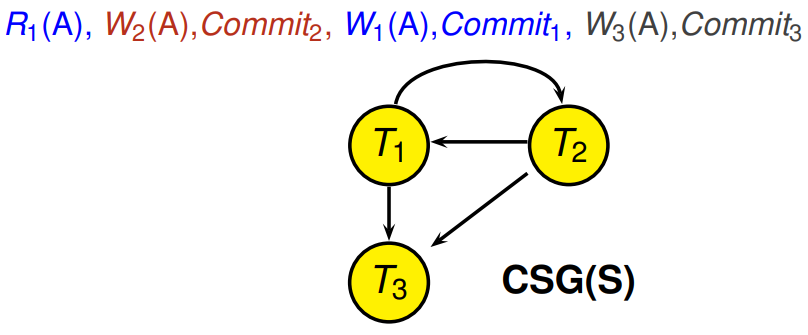
\includegraphics[width=7cm, height =2cm]{csg.png}


\textbf{ACID}
\begin{itemize}
  \item \textbf{Atomicity} Either all actions of a transaction are committed or none are
  \item \textbf{Consistency} Each transaction is consistent and DB begins in a consistent state $\rightarrow$ DB ends in a consistent state
  \item \textbf{Isolation} Execution of one xact is isolated from other Xacts 
  \item \textbf{Durability} Once a transaction is committed, its effects persists
  \item Concurrency control ensures isolation 
  \item Recovery manager ensures atomicity and durabilitt
  \item Consistency is ensured by constraints, cascades and triggers
\end{itemize}


\textbf{Schedules} \\
\begin{itemize} 
  \item \textbf{Cascading aborts} $T_i$ read from $T_j$ $\rightarrow$ $T_j$ aborts $\rightarrow$ $T_i$ aborts. This requires high book keeping efforts, so we turn to recoverable schedules instead.
  \item \textbf{Recoverable} $\forall T \in S$ T2 must commit after T1 if T2 reads from T1 (or T2 aborts before T1). Can still have cascading aborts. Is compulsory. 
  \item \textbf{Cascadeless} Whenever $T_i$ reads from $T_j$ in S, Commit must precede this action. Desirable, not compulsory.
  \item Theorem 4: Cascadeless $\rightarrow$ Recoverable (not iff)
  \item \textbf{Recovery with before image} Store the before image before write, restore this before image if write aborts. This can lead to \textbf{lost update} anomaly if the before image overwrites another Xact's write.
  \item \textbf{Strict}  to use before-images, $\forall W_i(O) \in S$, O is not read or written by another Xact until Ti either aborts or commits. This ensures no lost update anomaly during recovery.
  \item Strict schedules allows recovery using before images to be more efficient but restricts concurrency
  \item Theorem 5: Strict $\rightarrow$ Cascadless (not iff)
\end{itemize}

% Lecture 8
\subsection{L8: Concurrency Control}

\textbf{Lock based concurrency control} \\ 
\begin{itemize}
  \item If lock request is not granted, then T becomes blocked and gets added to O's request queue
\end{itemize}

\textbf{2PL} \\
\begin{itemize} 
  \item To read an object O, a Xact must hold a S-lock or X-lock on O 
  \item To write to an object O, a Xact must hold a X-lock on O 
  \item Once a Xact releases a lock, the Xact can't request any more locks
  \item Theorem 1: 2PL is conflict serializable
\end{itemize}

\textbf{Strict 2PL} \\
\begin{itemize}
  \item A Xact must hold on to locks until Xact commits or aborts
  \item Theorem 2: Strict 2PL is strict and conflict serializable
  \item Strict 2PL prevents cascading rollback and deadlock and ensures recoverability
\end{itemize}

\textbf{Anomalies not dealt by strict 2PL} \\
\begin{itemize}
  \item \textbf{Phantom Read:} T1 reads a set of objects, T2 inserts a new object in that set, T1 reads the set again and gets a different set of objects. 2PLS cannot prevent this as locks are held at the object level.
  \item Solved by \textbf{predicate locking}, which is done in practice by \textbf{index locking}
\end{itemize}
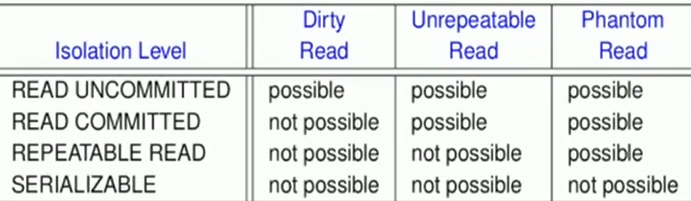
\includegraphics[width=7cm, height =1.5cm]{ansi_iso.png}

\textbf{Deadlock Detection} \\
\begin{itemize}
  \item Waits-for graph (WFG) → Deadlock is detected if WFG has a cycle. ($V_i, V_j \rightarrow T_i waits-for T_j$)
  \item Breaks a deadlock by aborting a Xact in cycle
  \item Alt: timeout mechanism 
\end{itemize}

\textbf{Deadlock Prevention} \\
\begin{itemize}
  \item Each Xact is assigned a timestamp when it starts
  \item Assume older (smaller time stamp) Xacts have higher priority than younger Xacts
  \item Tie between blocked/restarted xact brokered by priority, original timestamp is maintained to prevent starvation
  \item \textbf{Wait-die} Higher priority waits for lower priority, lower priority dies if higher priority holds lock (lower never waits)
  \item \textbf{Wound-wait} Higher priority kills lower priority, lower priority waits for higher priority to release lock (higher never waits)
\end{itemize}

% 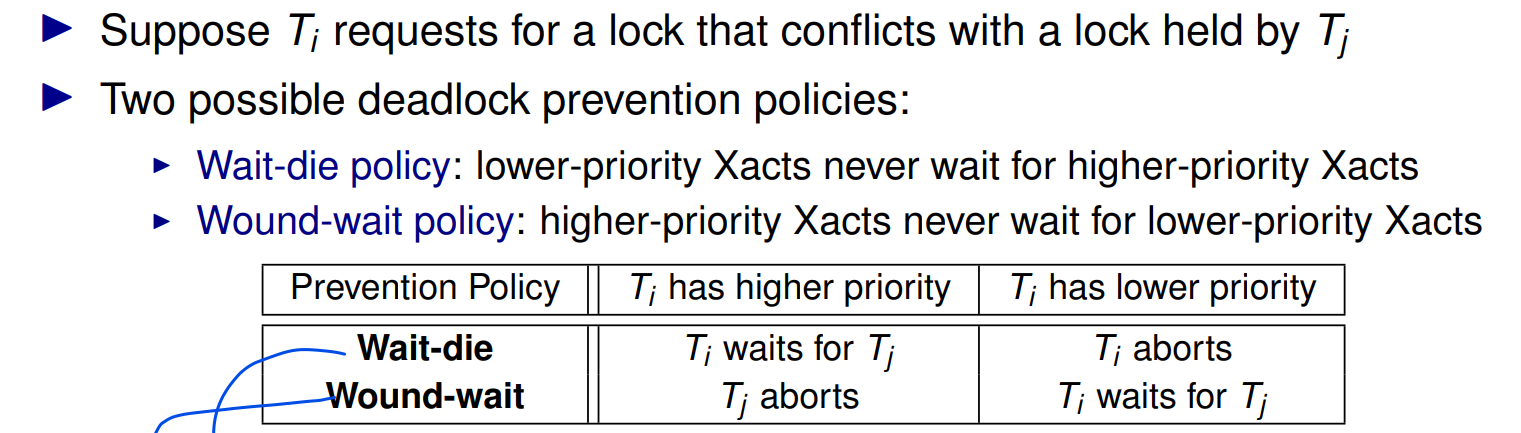
\includegraphics[width=7cm, height =2.5cm]{deadlock_prevention.png}

\textbf{Lock Conversion} \\
\begin{itemize}
  \item Allows for greater concurrency 
  \item Conversion is only allowed if the Xact has not released any lock 
  \item \textbf{Upgrade(A)} blocked if another Xact holds shared or exclusive lock on A
  \item \textbf{Downgrade(A)} allowed if Xact has not modified A and Xact has not released any lock
\end{itemize}

\textbf{Improve System Throughput} \\
\begin{itemize}
  \item Reduce Lock Granularity, Reduce time of lock being held, reduce hotspots in DB by changinge schema design
\end{itemize}

\textbf{Multi Version Serializable Schedle (MVSS)} \\
\textbf{Benefits} \\
\begin{itemize}
  \item $W_i(O)$ Creates new version
  \item Read-only Xact are not blocked by update xact (vice versa). Mono version (e.g. 2PL) blocks
  \item Read-only xacts are never aborted (no deadlocks due to Multi-version) or blocked
\end{itemize}

\begin{itemize}
  \item \textbf{multiversion view equivalent} if S and S' have the same set of read-from relationships
  \item i.e. Ri (xj ) occurs in S iff Ri (xj ) occurs in S'
  \item \textbf{Monoversion Schedule} each read action returns the most recently created object version. Not necessarily serializable
  \item \textbf{MVSS} if there exists a serial Monoversion schedule that is multiversion view equivalent to S
  \item Note that a MVSS is not necessarily conflict serializable schedule if it is not a valid monoversion schedule
  \item E.g. W1(x1), R2(x0), R2(y0), W1(y1), C1, C2 is MVSS with (T2, T1) but contains conflicting actions W1(x1) and R2(X0)
\end{itemize}

\textbf{Snapshot Isolation (SI) [NOT always serializable]} \\
\begin{itemize}
  \item Similar performance as Read Committed but does not suffer from lost update, unrepeatable read.
  \item Each Xact has a snapshot of the database at the start of the Xact and sees only versions from that snapshot and \textbf{its own writes}
  \item \textbf{FUW} T needs to acquire X-lock on O (if not - wait), and if O has been updated by a concurrent T' then T aborts
  \item \textbf{FCW} (no locks) before commiting T checks if O has been updated, abort if it has been updated
  \item \textbf{Write-skew anomaly}, not MVSS: $R_1(X_0), R_2(X_0), R_1(Y_1), R_2(Y_2), W_1(X_1),$ $ C_1, W_2(Y_2), C_2$
  \item \textbf{Read-only anomaly},not MVSS: $R_1(b), R_2(a),$\\$ W_1(b), C_1, R_2(b), W_2(a),R_3(a), R_3(b), C_3, C_2$
  \item \textbf{Non-MVSS SI} At least one cycle in DSG(s) with $T_i, T_j, T_k$ s.t $T_i,T_k$ are possibly the same xact, $T_i, T_j$ are concurrent with an edge $T_i$ rw $T_j$ and $T_j$ rw $T_k$
\end{itemize}

\textbf{Transaction Dependencies - Making SI serializable} \\
\begin{itemize}
  \item \textbf{WW} from T1 to T2: T1 commits some version of X and T2 writes the immediate successor
  \item \textbf{WR} from T1 to T2: T1 commits some version of X which is read by T2
  \item \textbf{RW} from T1 to T2: T1 reads some version of X and T2 commits the immediate successor
  \item \textbf{DSG} V = {xacts}, E = {Dependencies}, use --$>$ for concurrent transactions and $\rightarrow$ for non-concurrent
\end{itemize}

\textbf{Locking Granularity} \\ 
(Most coarse) DB, relation, page, tuple (Finest, more concurrency, less scalable) \\ 
Locks are acquired in a top down manner.
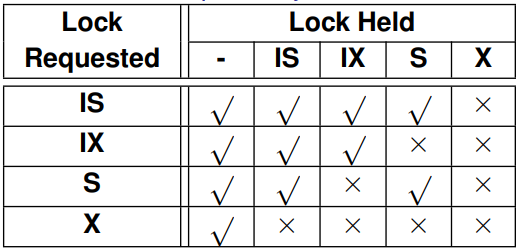
\includegraphics[width=4cm, height =1cm]{multigranular_locks.png}


\subsection{L9-Crash Recovery}
\textbf{Policies} \\
\begin{itemize}
  \item \textbf{Steal:} Allows dirty pages to be written to disk before commit
  \item \textbf{Force:} Requires all dirty pages to be written to disk when commit
  \item No-steal: no undo, Force: no redo. Pgsql uses steal and no-force
\end{itemize}

\textbf{Restart: analysis, redo, undo} \\
\begin{itemize}
  \item Analysis: identifies dirtied pool pages and active Xacts at time of crush
  \item Redo: redo actions to restore db to pre-crush
  \item Undo: undo actions of Xacts that did not commit
\end{itemize}

\textbf{Analysis: Xact table} \\
\begin{enumerate}
  \item When the first log record is created, create a new entry T with status U
  \item Update lastLSN for T to be r's LSN
  \item Remove T if end log is seen
\end{enumerate}

\textbf{Analysis: Dirty Page Table} \\
\begin{enumerate}
  \item New dirtied page will be added to the DPT with recLSN=r.LSN
  \item Remove entry when it is flushed to disk
\end{enumerate}

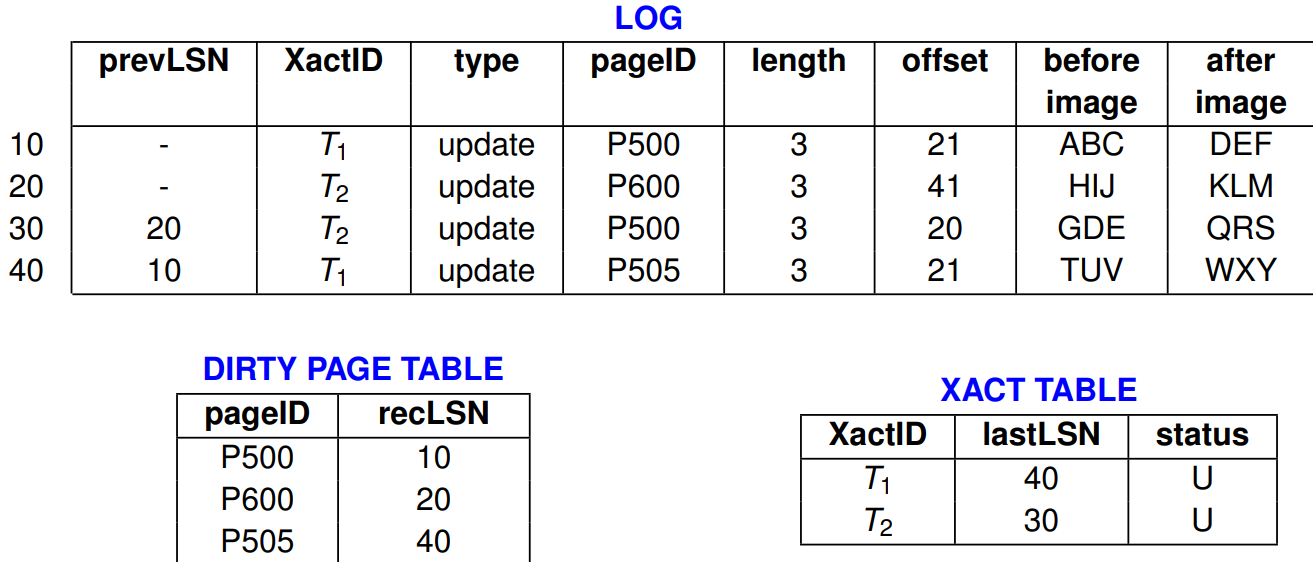
\includegraphics[width=7cm, height =2cm]{analysis_log.png}

\textbf{Redo Phase (DPT)} \\
\begin{enumerate}
  \item Redo LSN = min(recLSNs), then fetch page LSN, 
  \item if r.LSN $>$ pageLSN and Page is in DPT, redo
  \item Update pageLSN to r.LSN
\end{enumerate}

\textbf{Undo Phase (TT)} \\
\begin{enumerate}
  \item Start from largest LSN from L
  \item if update, create CLR with undoNextLSN=r's prevLSN, update-L-TT(r.prevLSN)
  \item if CLR, update-L-TT(r.undoNextLSN)
  \item update-L-TT(lsn): add lsn to L if lsn not null, else add end log record for T and remove it from TT
\end{enumerate}

\textbf{Checkpointing} \\
\begin{itemize}
  \item Normal(no ECPLR): CPLR's TT, empty DPT
  \item Fuzzy: BeginCPLR's TT and BCPLR's DPT  
\end{itemize}

\end{multicols}
\end{document}